\documentclass[11pt,letterpaper]{article}

\usepackage[margin=1in]{geometry}
\usepackage{amsmath,amssymb,bm}
\usepackage{siunitx}
\usepackage{booktabs}
\usepackage{graphicx}
\usepackage{xcolor}
\usepackage{hyperref}
\usepackage{enumitem}
\usepackage{microtype}
\usepackage{setspace}
\usepackage[numbers,sort&compress]{natbib}

\hypersetup{
  colorlinks=true,
  linkcolor=blue!50!black,
  citecolor=blue!50!black,
  urlcolor=blue!50!black
}

\sisetup{per-mode=symbol, separate-uncertainty=true}

\newcommand{\gtt}{g^{(2)}}
\newcommand{\avg}[1]{\left\langle #1 \right\rangle}

\title{Angular and Rotation-Rate Scaling of Speckle\\
Intensity Autocorrelations from a Rotating Diffuser}
\author{Gantulga Gankhuyag and E.~Landahl\\[0.4em]
\large\textit{Draft --- based on data acquired 24~July~2026}}
\date{\today}

\begin{document}
\maketitle

\begin{abstract}
We measure normalized intensity autocorrelations of laser light scattered from a
rotating ground-glass diffuser using a single-photon counting module and an
FPGA-based logarithmic multi-$\tau$ correlator. Traces are recorded at scattering
angles of approximately $0^\circ$, $10^\circ$, $15^\circ$, and $20^\circ$ for several
rotation periods. On a logarithmic delay axis the decays are well described by a
four-parameter complementary-error-function (erfc) sigmoid in $\ln\tau$, from which
we extract a midpoint time $\tau_{50}$. At fixed angle, $1/\tau_{50}$ increases
linearly with angular speed $\omega$, consistent with the prediction that
diffuser angular displacement $\omega\tau$---not absolute time---governs
decorrelation. The slope of that relation grows approximately in proportion to
$\sin\theta$ for the well-aligned off-axis angles, in qualitative agreement with
far-field models of rigidly rotating speckle. A nominal forward-scattering run
still shows finite decay; we omit it from the $\sin\theta$ fit because of
imperfect on-axis alignment. We summarize what is established by
these data, how it compares with classical rotating-diffuser literature, and what
measurements would most usefully extend the result.
\end{abstract}

\section{Introduction}
\label{sec:intro}

When coherent light illuminates a rough surface, the scattered field forms a
speckle pattern whose spatial and temporal statistics encode the surface
structure and its motion~\cite{GoodmanSpeckle,GoodmanStatistical}. For an
in-plane rotating diffuser, the pattern evolves as new regions of the rough
surface enter the illuminated spot and as the far-field interference pattern
rotates or translates. Intensity fluctuations at a fixed detector therefore
decorrelate on a time scale set by the rotation rate and by the optical
geometry~\cite{Saleh1975,Churnside1982,Yoshimura1986,Yura1998}.

This physics is both a classical metrology problem---speckle correlation and
zero-crossing methods have long been used to infer surface
velocity~\cite{Saleh1975,Takai1980}---and a practical tool. Rotating or translating
diffusers are routinely used to reduce spatial coherence, homogenize beams, and
synthesize pseudo-thermal light~\cite{GoodmanSpeckle}. More recently, the same
spatiotemporal intensity fields have been discussed as controllable random
optical drives for thermal-transport and system-identification
experiments. In all of those settings one needs a quantitative map from
rotation rate and observation angle to the temporal spectrum of the intensity.

The present experiment is a focused test of the simplest scaling predictions.
If the diffuser presents a fixed sequence of scattering configurations as it
rotates, then changing the angular speed $\omega$ should only change the
\emph{playback rate} of that sequence. At fixed scattering angle $\theta$,
normalized correlation curves should then collapse when plotted against the
angular displacement $\omega\tau$, which implies
\begin{equation}
  \tau_c(\theta,\omega)
  =
  \frac{\Delta\theta_c(\theta)}{\omega},
  \qquad\text{or equivalently}\qquad
  \frac{1}{\tau_c}
  \propto
  \omega.
  \label{eq:omega_scaling}
\end{equation}
Here $\Delta\theta_c$ is a characteristic diffuser rotation angle required to
decorrelate the detected intensity. Idealized far-field models of
\emph{centered}, rigidly rotating circular illumination further predict that
the correlation time shortens with angle roughly as
$1/\sin\theta$~\cite{Churnside1982,Yura1998}, so that the slope in
Eq.~\eqref{eq:omega_scaling} itself should increase with $\sin\theta$.

Our goals in this draft are deliberately limited. We (i)~acquire multi-$\tau$
photon autocorrelations over a grid of angles and rotation periods,
(ii)~fit each curve with a log-delay sigmoid matched to the multi-$\tau$
sampling, (iii)~test Eq.~\eqref{eq:omega_scaling}, and (iv)~compare the
extracted slopes with a $\sin\theta$ trend. We do \emph{not} yet claim a full
reconstruction of the sample-plane spatiotemporal spectrum, nor a precision
measurement of illuminated diameter.

\section{Background}
\label{sec:background}

\subsection{Intensity autocorrelation}

Let $I(t)$ be the photocount-derived intensity at a fixed detector. The
normalized second-order correlation commonly used in dynamic light
scattering~\cite{BernePecoraBook,Schatzel1990} is
\begin{equation}
  \gtt(\tau)
  =
  \frac{\avg{I(t)\,I(t+\tau)}}{\avg{I(t)}^2}.
  \label{eq:g2}
\end{equation}
For a stationary process, $\gtt(\tau)\to 1$ at long delay. The intercept
$\gtt(0)-1$ is the measured speckle contrast $\beta$; it is reduced below the
ideal single-mode value of unity by finite detector area, polarization mixing,
and temporal averaging~\cite{GoodmanSpeckle}.

\subsection{Rotating-diffuser expectations}

Saleh, Tavolacci, and Soper demonstrated velocity measurement from
rotating-object speckle correlations~\cite{Saleh1975}. Churnside analyzed
speckle from a rotating diffuse object in detail~\cite{Churnside1982}.
Yoshimura and coworkers distinguished rotational motion of the pattern from
speckle ``boiling''~\cite{Yoshimura1986}. Yura, Rose, and Hanson gave ABCD-system
expressions for in-plane rotation~\cite{Yura1998}. In the idealized limit of a
circular pupil centered on the rotation axis, the short-delay field correlation
takes a jinc form and the intensity correlation follows from the Siegert
relation, yielding
\begin{equation}
  \gtt(\tau)-1
  \approx
  \beta
  \left[
    \frac{2J_1(X)}{X}
  \right]^2,
  \qquad
  X
  \propto
  D\,\omega\sin\theta\,\tau/\lambda,
  \label{eq:jinc}
\end{equation}
with illuminated diameter $D$ and wavelength $\lambda$. Equation~\eqref{eq:jinc}
implies both the $\omega^{-1}$ scaling of Eq.~\eqref{eq:omega_scaling} and an
angle factor $\sin\theta$. Off-axis illumination, beam nonuniformity, and
surface boiling replace or supplement rigid rotation with additional
decorrelation channels~\cite{Yoshimura1986,Yura1998}.

\subsection{Why an erfc$(\ln\tau)$ fit?}

Our correlator returns lags on an approximately logarithmic grid. On a
$\log\tau$ axis the measured decays look like smooth sigmoids rather than pure
exponentials. A convenient phenomenological model, already used in our laboratory
for multi-$\tau$ dynamic-light-scattering traces, is
\begin{equation}
  \gtt(\tau)
  =
  A\,\mathrm{erfc}\!
  \left(
    \frac{\ln\tau-B}{C_w}
  \right)
  +
  D,
  \label{eq:erfc}
\end{equation}
where $\mathrm{erfc}$ is the complementary error function. The midpoint
\begin{equation}
  \tau_{50}=e^{B}
\end{equation}
is a robust characteristic time on the log-delay axis. The parameter $C_w$ sets
the transition width in units of $\ln\tau$, and the step height $2A$ estimates
the contrast $\beta$ when the baseline $D\approx 1$. This form does not replace
a first-principles jinc model; it is a data-reduction tool well matched to
log-spaced sampling. Pilot comparisons on representative runs showed that a
single exponential ($\alpha=1$ stretched exponential) is a poor description of
these diffuser curves, whereas Eq.~\eqref{eq:erfc} and free-shape stretched
exponentials both perform well. Ideal jinc$^2$ curves alone leave systematic
Airy-lobe residuals and are not used for the scaling analysis below.

\section{Experiment}
\label{sec:experiment}

\subsection{Apparatus}

A diode laser (operating near \SI{650}{\nano\meter}, drive
\SI{3.31}{\volt}/\SI{0.033}{\ampere}) was focused onto a rotating ground-glass
diffuser mounted at the center of a diffractometer-style rotation stage. The
diffuser grit was not recorded for this run and is left unspecified. Scattered
light was collected into a Thorlabs single-photon counting module with a
\SI{20}{\micro\meter} active diameter. An iris kept the mean count rate of order
\SI{1}{\mega\hertz} (measured rates in the present files span roughly
\SIrange{1}{2.3}{\mega\hertz}). Collection optics beyond the iris were not fully
characterized in this first survey.

Photon arrival times were processed by a custom FPGA logarithmic multi-$\tau$
binary autocorrelator clocked at $f=\SI{12}{\mega\hertz}$. Host software
(\texttt{simple\_multitau.m}, a single-angle simplification of a multi-angle
acquisition code) requested \SI{10}{\second} acquisitions, read the correlation
bins over SPI, and saved Octave text exports together with a semilog-$x$
preview figure.

\subsection{Run matrix}

Autocorrelations were taken at four nominal scattering angles---$20^\circ$,
$15^\circ$, $10^\circ$, and $0^\circ$---with six rotation periods at each angle
(two periods share the label \texttt{test027} at $15^\circ$). Early unlabeled
filenames correspond to $20^\circ$. Rotation periods $T_{\mathrm{rot}}$ were timed
with a stopwatch for one revolution and encoded in the filenames; angular speed
is taken as
\begin{equation}
  \omega = \frac{2\pi}{T_{\mathrm{rot}}}.
\end{equation}
The nominal $0^\circ$ setting required a very small iris for on-axis count-rate
control and was only roughly aligned; we treat those runs as a poorly
constrained \emph{small angle}, not as true forward scattering.

\subsection{Normalization}

The correlator returns coincidence counts divided by the total photon count.
With clock duration $T_{\mathrm{clk}}$ (in cycles) and total counts $N$, the
mean occupancy per clock cycle is $\langle n\rangle=N/T_{\mathrm{clk}}$. We form
\begin{equation}
  \gtt(\tau)
  =
  \frac{\mathrm{AC}(\tau)}{\langle n\rangle}
  =
  \mathrm{AC}(\tau)\,\frac{T_{\mathrm{clk}}}{N},
\end{equation}
so that the long-delay baseline approaches unity. The first ten lags
($\tau\lesssim\SI{0.8}{\micro\second}$) show a sharp afterpulsing rise and are
excluded from all fits.

\section{Data analysis}
\label{sec:analysis}

Each trace was fitted to Eq.~\eqref{eq:erfc} over
$\SI{0.8}{\micro\second}\lesssim\tau\le\SI{0.1}{\second}$ by nonlinear least
squares. Parameter uncertainties were estimated by residual bootstrap
(400 resamples), which is more conservative than formal covariance errors when
residuals contain smooth systematic structure. From each fit we retain
$\tau_{50}$, $\beta\approx 2A$, $C_w$, and the baseline $D$.

At each fixed angle we then fit
\begin{equation}
  \frac{1}{\tau_{50}}
  =
  m\,\omega + b
  \label{eq:line}
\end{equation}
with a floated intercept $b$. Ideal playback-rate scaling predicts $b\approx 0$
and a slope $m=1/\Delta\theta_c$. Finally we plot the floated slopes $m(\theta)$
against $\sin\theta$ for the off-axis angles and fit a straight line with floated
intercept.

\section{Results}
\label{sec:results}

\subsection{Shape of individual correlations}

Figure~\ref{fig:fits} shows three representative fits at mid-range rotation
periods for $10^\circ$, $15^\circ$, and $20^\circ$. In each case the erfc$(\ln\tau)$
model captures the plateau, the sigmoidal shoulder on the log-delay axis, and
the return to baseline. Extracted midpoints are of order
\SIrange{0.7}{2}{\milli\second} for these examples, with bootstrap
uncertainties at the percent level or better. Contrast $\beta$ increases from
about $0.19$ at $10^\circ$ to about $0.24$ at $20^\circ$ in these exemplars,
consistent with the broader data set.

\begin{figure}[t]
  \centering
  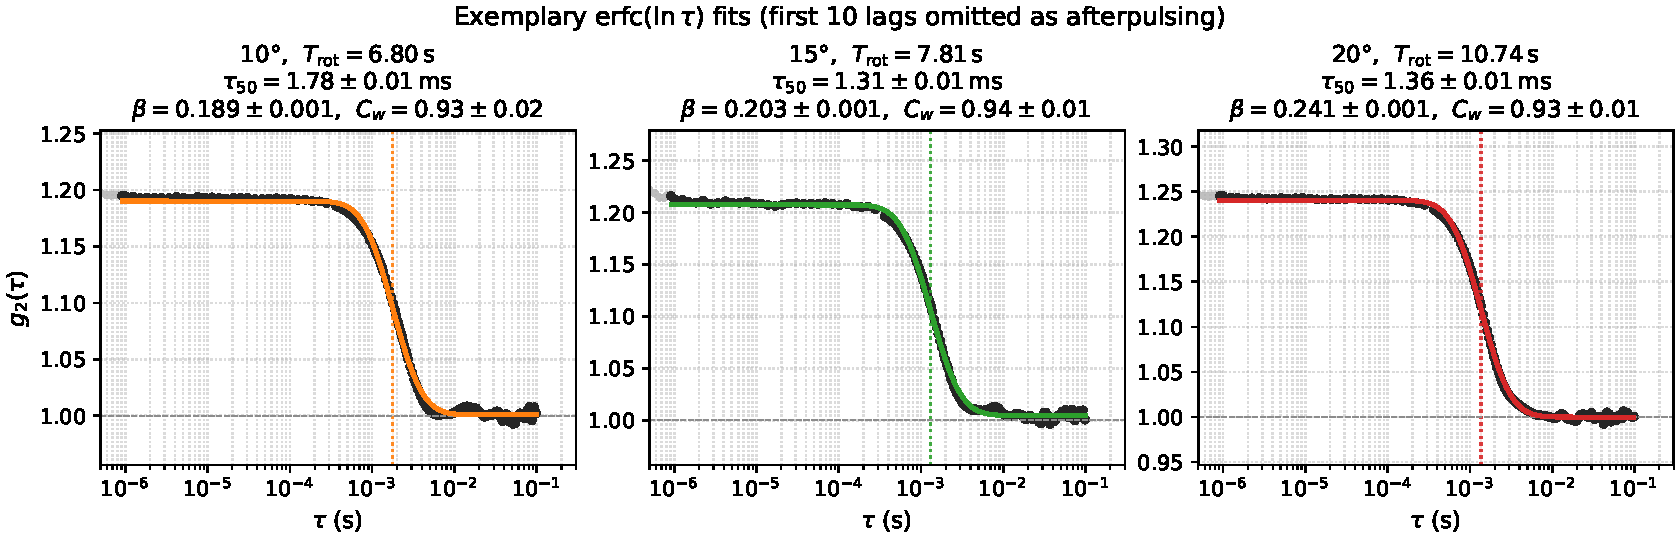
\includegraphics[width=\textwidth]{figures/fig_exemplary_fits.pdf}
  \caption{Exemplary normalized autocorrelations and erfc$(\ln\tau)$ fits at
  three scattering angles. Grey early points are omitted from the fit
  (afterpulsing). The dotted vertical line marks $\tau_{50}$; the shaded band
  is the bootstrap uncertainty on $\tau_{50}$.}
  \label{fig:fits}
\end{figure}

\subsection{Scaling with rotation rate}

Figure~\ref{fig:omega} plots $1/\tau_{50}$ versus $\omega$ for all angles, with
a separate floated-intercept line at each angle. The off-axis families
($10^\circ$--$20^\circ$) are strikingly linear. Intercepts are small compared with
the span of the data, so the leading behavior is the through-origin relation
predicted by Eq.~\eqref{eq:omega_scaling}. Faster rotation (larger $\omega$)
systematically yields faster decorrelation (larger $1/\tau_{50}$), in quantitative
proportion at fixed angle.

\begin{figure}[t]
  \centering
  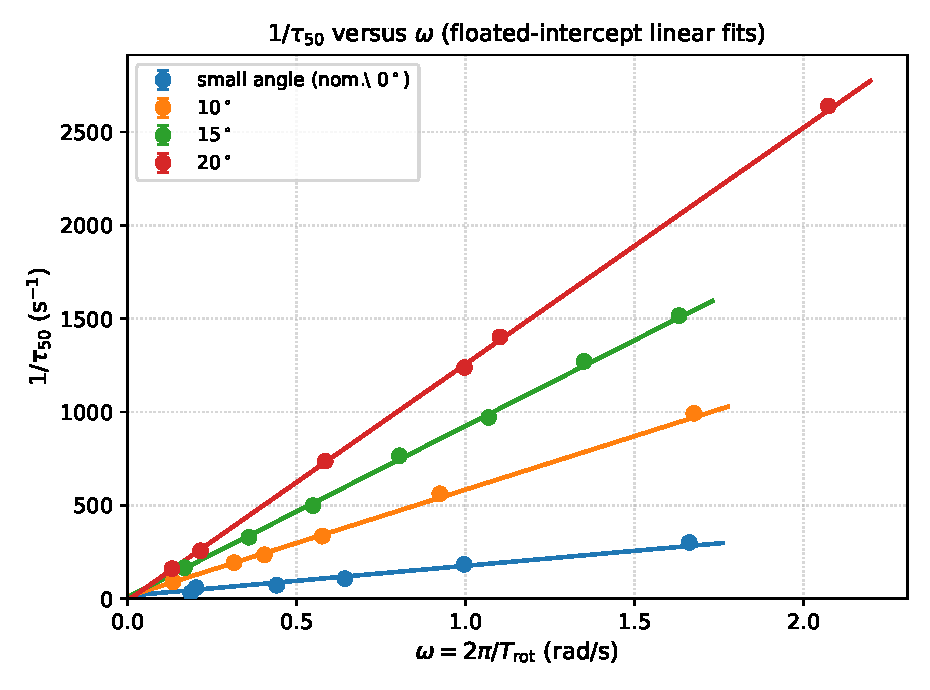
\includegraphics[width=0.72\textwidth]{figures/fig_inv_tau50_vs_omega.pdf}
  \caption{Inverse midpoint time versus angular speed. Solid lines are
  weighted linear fits with floated intercepts. Error bars are smaller than
  the markers in most cases.}
  \label{fig:omega}
\end{figure}

Table~\ref{tab:slopes} lists the floated slopes. Equivalent angular
decorrelation scales $\Delta\theta_c\equiv 1/m$ (using the origin-forced slope
from the companion analysis) shrink from roughly $0.10^\circ$ at $10^\circ$ to
$0.05^\circ$ at $20^\circ$: less diffuser rotation is needed to refresh the
speckle at larger scattering angle.

\begin{table}[t]
\centering
\caption{Floated-intercept slopes of $1/\tau_{50}=m\omega+b$. Uncertainties are
from the weighted line fit using bootstrap errors on $\tau_{50}$.}
\label{tab:slopes}
\begin{tabular}{lS[table-format=4.1]
                S[table-format=2.1]
                S[table-format=4.1]
                S[table-format=2.1]}
\toprule
{Angle} & {$m$} & {$u(m)$} & {$b$~(s$^{-1}$)} & {$u(b)$} \\
\midrule
small (nom.\ $0^\circ$) & 160.6 & 1.9 & 15.4 & 0.7 \\
$10^\circ$ & 572.6 & 3.0 & 11.9 & 0.9 \\
$15^\circ$ & 917.8 & 3.8 & 7.7 & 1.7 \\
$20^\circ$ & 1266.6 & 3.8 & -9.7 & 1.2 \\
\bottomrule
\end{tabular}
\end{table}

\subsection{Scaling with angle}

Figure~\ref{fig:sin} shows the floated slopes versus $\sin\theta$ for
$10^\circ$, $15^\circ$, and $20^\circ$ only. A weighted line with floated intercept gives
\begin{equation}
  m(\theta)
  =
  (4.12\pm 0.03)\times 10^{3}\,\sin\theta
  -
  (1.44\pm 0.07)\times 10^{2}.
\end{equation}
The dominant trend is still an increase with $\sin\theta$, as expected if
$\tau_{50}$ tracks the combination $\omega\sin\theta$ that appears in idealized
far-field models~\cite{Churnside1982,Yura1998}---even though the detailed
jinc$^2$ \emph{shape} is not required for this scaling test. The modest
negative intercept shows that a pure through-origin $\propto\sin\theta$ law is
only approximate over this angular window.

The nominal near-forward runs are omitted from Fig.~\ref{fig:sin}. They still
exhibit finite decorrelation and a shallow $1/\tau_{50}$--$\omega$ slope
(Table~\ref{tab:slopes}), which is expected if the detector is not at true
forward scattering, if the beam is not centered on the rotation axis, or if
boiling/wobble contribute weakly angle-dependent
dynamics~\cite{Yoshimura1986}. Given the documented rough alignment of those
runs, we treat them as a geometry diagnostic rather than part of the
$\sin\theta$ test.

\begin{figure}[t]
  \centering
  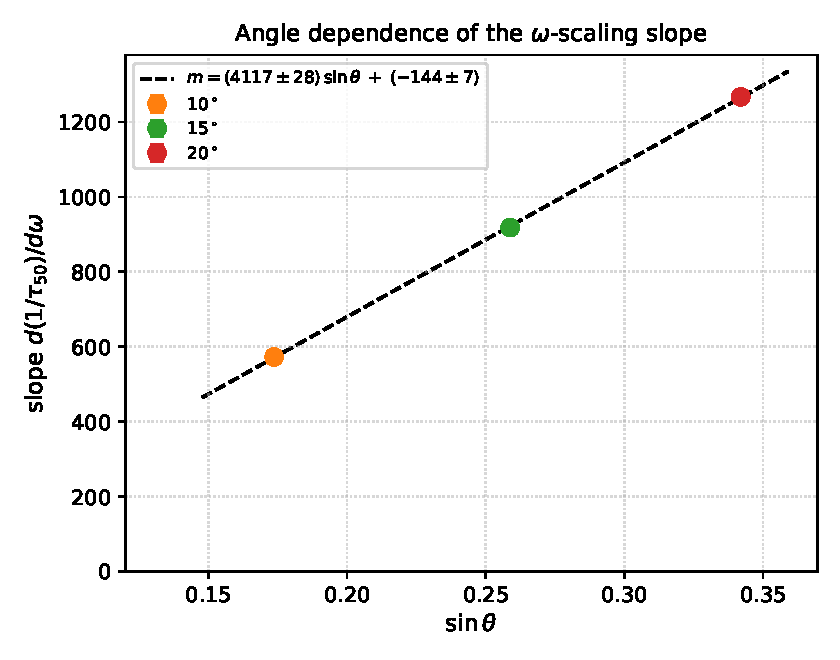
\includegraphics[width=0.62\textwidth]{figures/fig_slopes_vs_sintheta.pdf}
  \caption{Floated slopes from Fig.~\ref{fig:omega} versus $\sin\theta$ for
  $10^\circ$, $15^\circ$, and $20^\circ$. The dashed line is a weighted linear fit with
  floated intercept. The nominal small-angle runs are omitted.}
  \label{fig:sin}
\end{figure}

\section{Comparison with theory and prior work}
\label{sec:compare}

\paragraph{Agreement.}
The data affirm the playback-rate hypothesis of Eq.~\eqref{eq:omega_scaling} at
fixed angle and a clear $\sin\theta$ increase of the rate constant for
$10^\circ$--$20^\circ$. Both are standard expectations from rotating-diffuser
speckle theory~\cite{Churnside1982,Yura1998} and from earlier correlation-based
velocimetry~\cite{Saleh1975,Takai1980}. The practical advance here is a compact,
photon-counting multi-$\tau$ survey that makes the two-parameter scaling
$(\omega,\theta)$ visible in a single afternoon's run matrix, with modern
log-lag instrumentation and a fit function matched to that lag grid.

\paragraph{Limits of the present comparison.}
We have not yet determined the illuminated diameter $D$ independently, so we do
not convert the measured $k$ into a precision test of the prefactor in
Eq.~\eqref{eq:jinc}. Collection optics are incompletely specified, so absolute
contrast $\beta$ should not be over-interpreted. The erfc$(\ln\tau)$ midpoint
$\tau_{50}$ is not identical to the $1/e$ time of a jinc$^2$ or stretched
exponential; it is a consistent empirical clock for scaling tests, not a
claim that the microscopic correlation equals an error function.

\paragraph{What is new relative to classical papers.}
Classical studies established the mechanisms and often emphasized velocity
extraction or imaging-geometry taxonomy~\cite{Saleh1975,Churnside1982,Yoshimura1986}.
The present draft's contribution is narrower but concrete: a clear experimental
collapse of $\tau_{50}(\omega)$ at several angles on a photon-counting FPGA
correlator, plus a direct $\sin\theta$ test of the resulting slopes, including an
honest treatment of a misaligned near-forward channel.

\section{Conclusions and outlook}
\label{sec:conclusions}

Within the off-axis data set, prediction and measurement agree on two central
points: (1)~decorrelation rates scale linearly with rotation speed at fixed
angle, and (2)~those rates increase with $\sin\theta$. A phenomenological
erfc$(\ln\tau)$ fit provides stable $\tau_{50}$ values for that test. The
near-forward runs remind us that geometry must be controlled before interpreting
small-angle residuals as intrinsic boiling.

The most impactful next experiments are, in our view:

\begin{enumerate}[leftmargin=1.6em]
  \item \textbf{Collapse of full curves}, not only $\tau_{50}$: plot
  contrast-normalized $\gtt$ against $\omega\tau$ (and against
  $\omega\tau\sin\theta$) to test shape invariance~\cite{Yura1998}.
  \item \textbf{Revolution echoes:} extend the lag window over one or more
  full periods to measure recurrence amplitude---a direct probe of rigid
  versus boiling dynamics~\cite{Yoshimura1986}.
  \item \textbf{Controlled beam offset $R$:} vary the illuminated radius from
  the axis to separate tangential-displacement scaling
  $\ell_c\sim R\omega\tau_c$ from pure angular scaling.
  \item \textbf{Camera measurement of} $\mathcal{S}_I(\mathbf{k},\omega)$ at
  the intended sample/heating plane, which single-point autocorrelations cannot
  fully determine.
  \item \textbf{Documented grit, spot size, and collection NA}, enabling a
  quantitative jinc or ABCD comparison rather than slope ratios alone.
\end{enumerate}

Items 1--3 stay within the present photon-correlator setup and would most
directly tighten the link between this data set and the classical theory.
Items 4--5 open the path from characterization of the diffuser drive to its use
as a calibrated stochastic optical field.

\section*{Acknowledgments}
We thank collaborators on the FPGA correlator and diffractometer infrastructure.
This draft describes analysis of the 24~July~2026 rotating-diffuser data set.

\bibliographystyle{unsrtnat}
\bibliography{refs}

\end{document}
